F\"ur die Bestimmung des Templates des korrelierten Untergrunds wird das Template des Signals von einer Verteilung invarianter Masse abgezogen.
Die Verteilung invarianter Masse kommt dabei ebenfalls aus der Monte Carlo Simulation, auf die das Analyseverfahren bis einschlie{\ss}lich der Absch\"atzung der unkorellierten Untergrunds, so wie bisher erl\"autert, angewandt wurde.
\begin{figure}[tp]
\centering
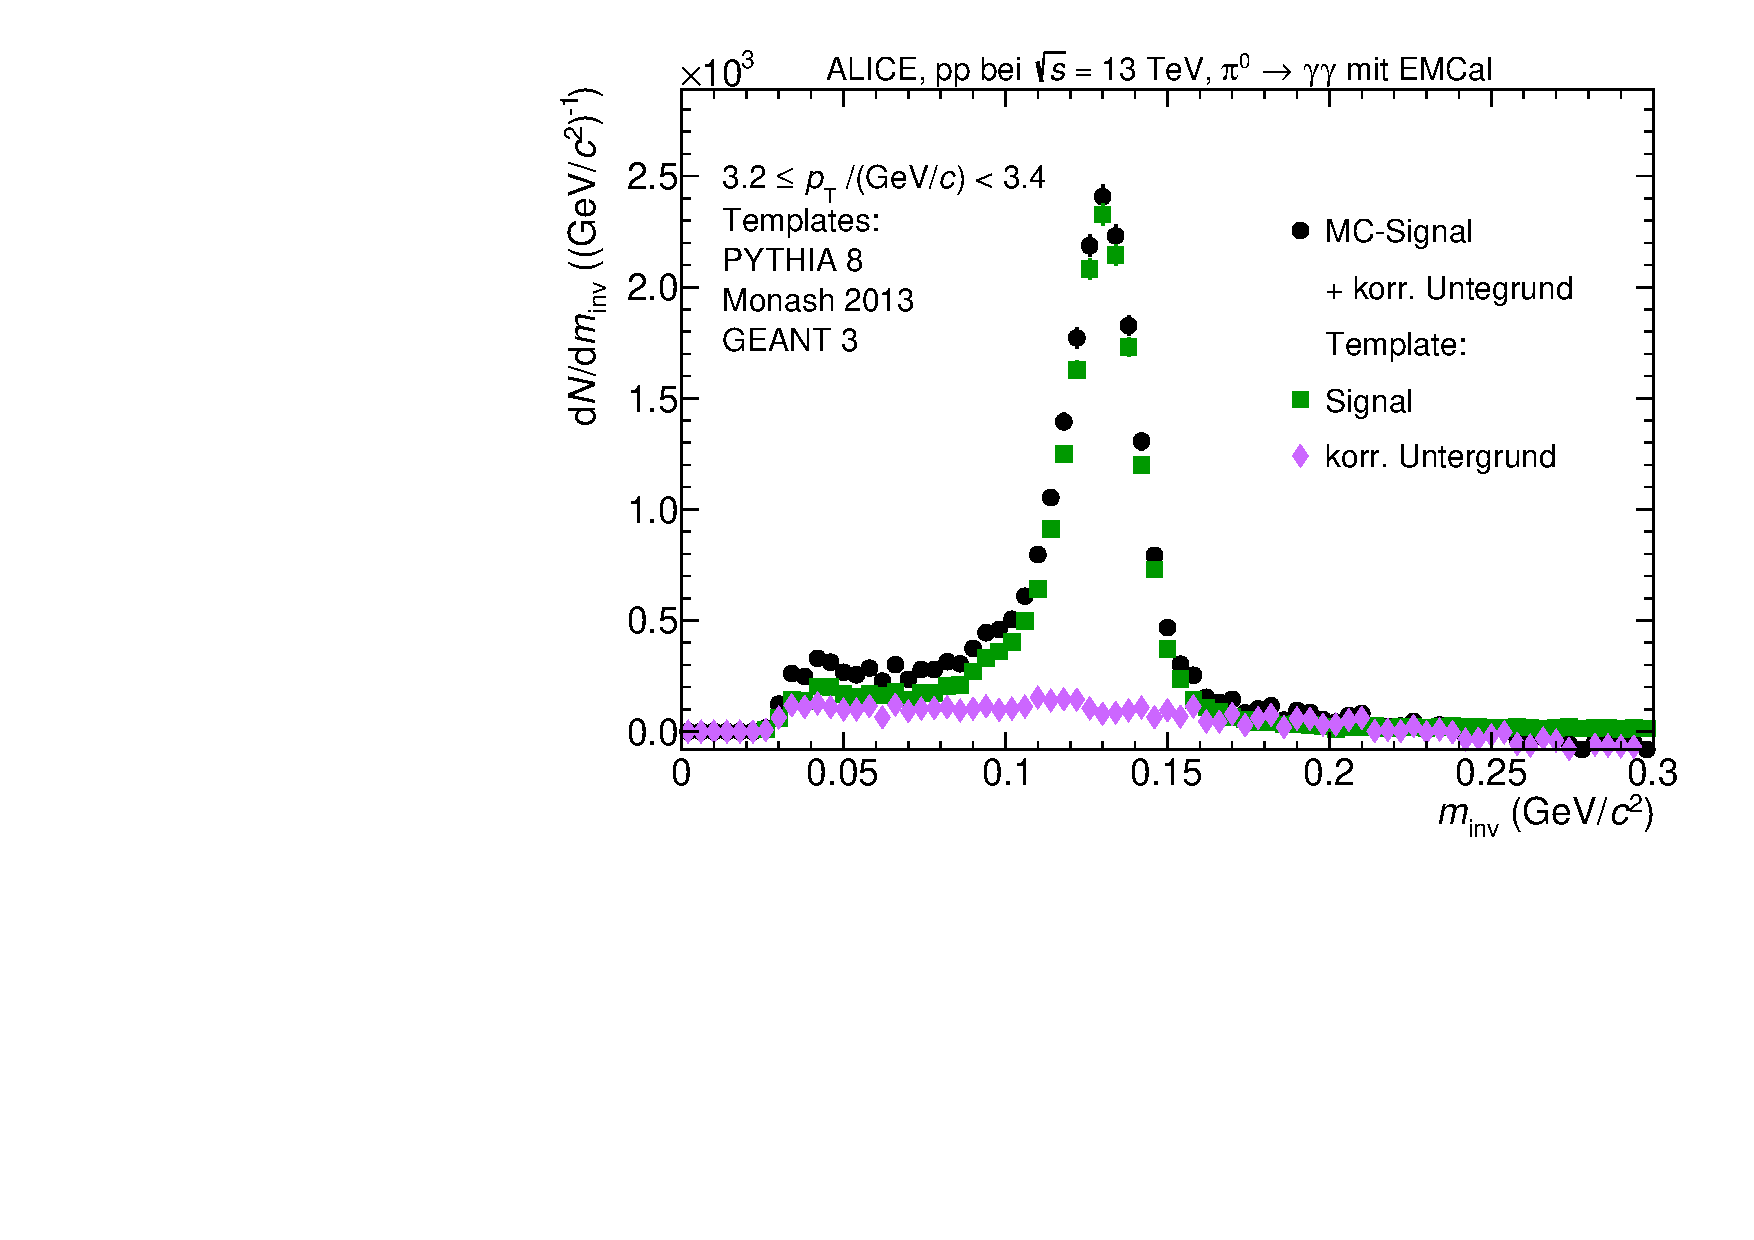
\includegraphics[width=.75\linewidth]{EntstehungUntergrund10_Data_2016.pdf}
\caption{.}
\label{fig:BkgTemp}
\end{figure}
\newline
Abbildung \ref{fig:BkgTemp} zeigt das Template des korrelierten Untergrunds in pink.
Zur Verdeutlichung sind ebenfalls das oben beschriebene Signal in schwarz und das Template des Signals in gr\"un eingezeichnet.
\newline
Da die statistische Unsicherheit im korrelierten Untergrund relativ gro{\ss} ausf\"allt verglichen mit der Anzahl an Eintr\"agen in der Verteilung der invarianten Masse, wird in dieser Arbeit der korrelierte Untergrund aus mehreren $p_\text{T}$-Intervallen zusammengefasst.
Dabei werden die Templates des korrelierten Untergrunds aus den $p_\text{T}$-Intervallen von $p_\text{T} \beq 1,8\text{ GeV}/c$ bis $p_\text{T} \leq 2,8\text{ GeV}/c$ aufgrund der geringen statistischen Unsicherheit benutzt.
Diese werden zun\"achst aufsummiert und auf die Anzahl der verwendeten $p_\text{T}$-Intervalle normiert.
\begin{figure}[tp]
\centering
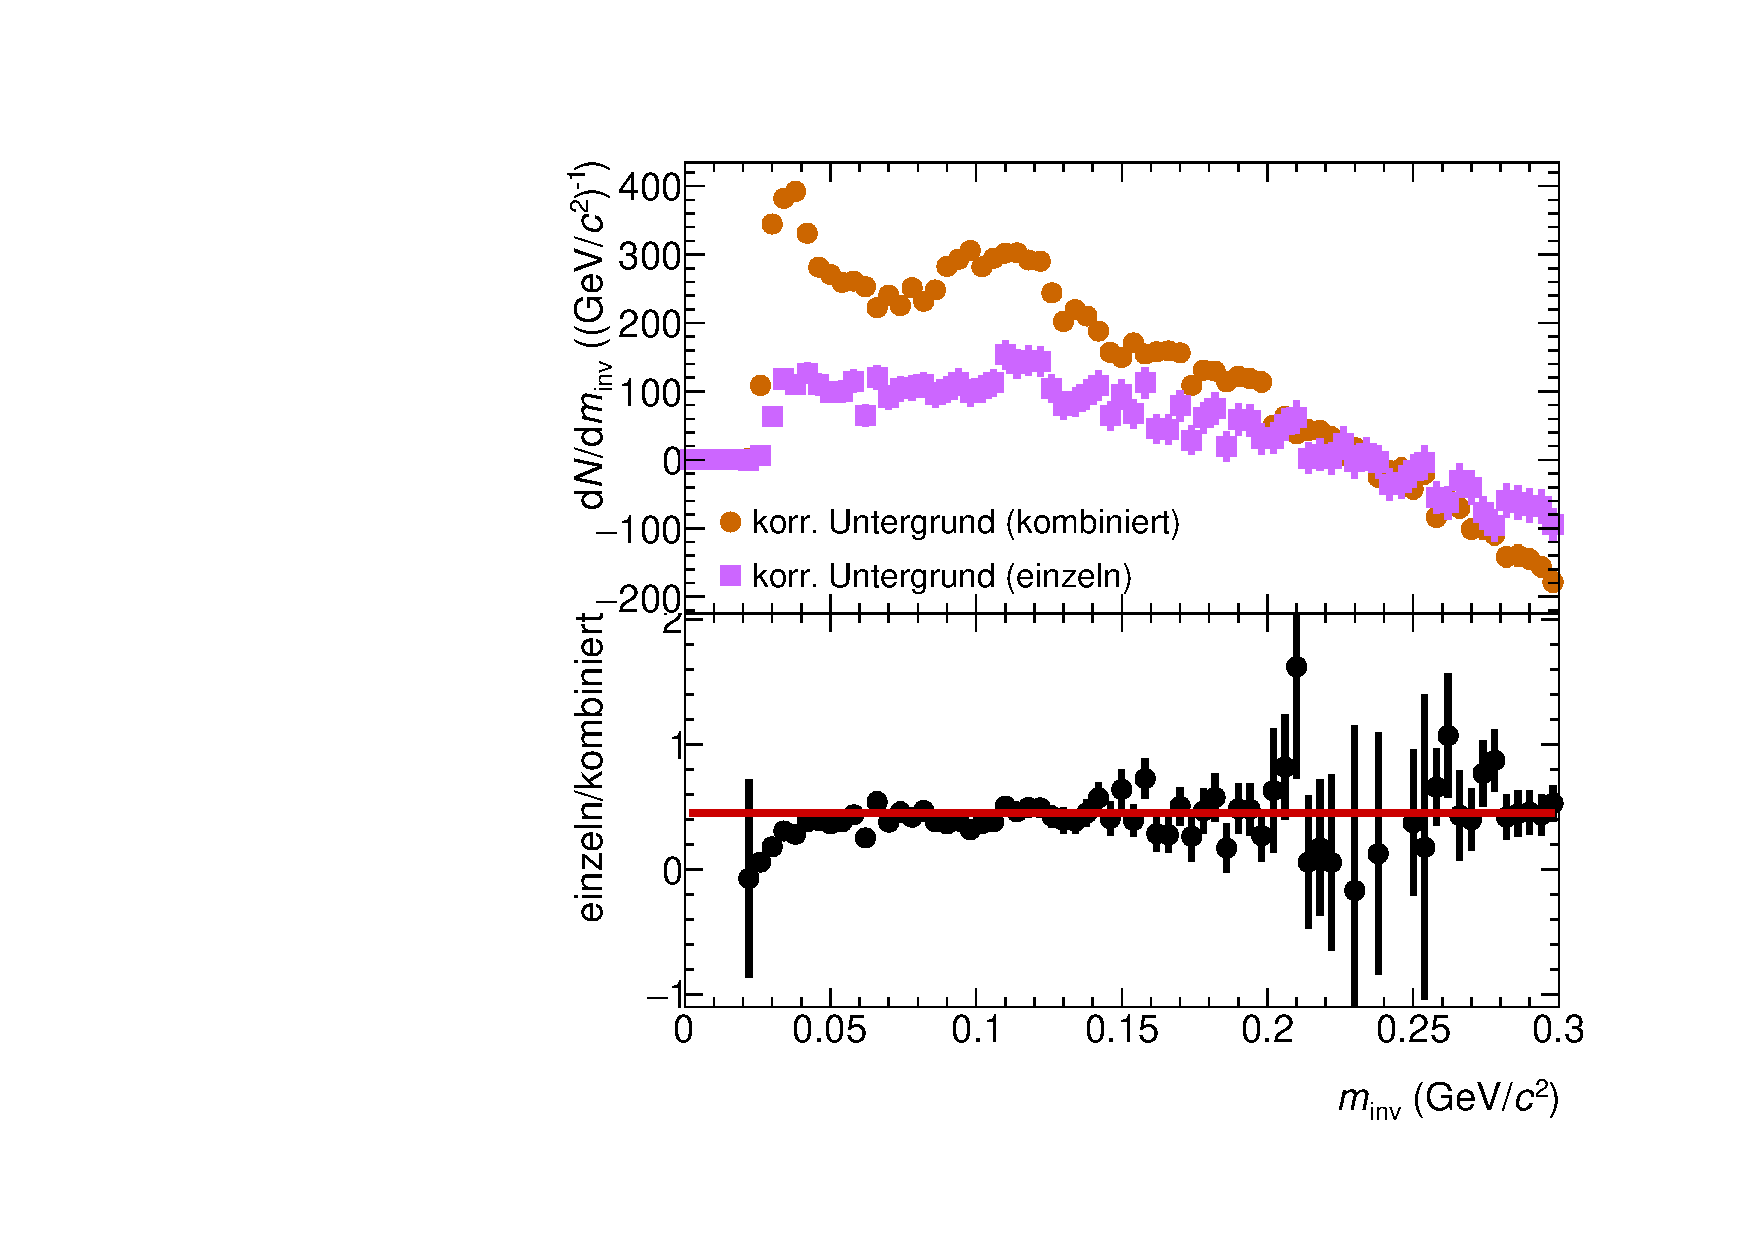
\includegraphics[width=.75\linewidth]{BackgroundWithRatio10_Data_2016.pdf}
\caption{.}
\label{fig:BkgTempRatio}
\end{figure}
\newline
Abbildung \ref{fig:BkgTempRatio} zeigt in pink ein kombiniertes Template des korrelierten Untergrunds und in gr\"un das Template des korrelierten Untergrunds f\"ur das $p_\text{T}$-Intervall $(3,2 - 3,4) (\text{GeV/}c)$.

\newline
Im Folgenden Abschnitt werden die beiden Templates so parametrisiert, dass sie das Signal nach Absch\"atzung des unkorrelierten Untergrunds bestm\"oglich beschreiben.